\section{Experimental Setup}

We have described details of the experimental setup in ref.\cite{Araoka:2011pw},
and in this paper we only discuss the issues which are relevant.

\subsection{K1.1Br Beamline}
\begin{itemize}
\item Designed and constructed for TREK experiment
\item 30 GeV proton + target, ESS for good particle separation (Max $K/\pi$ = 1)
\item highest intensity at 3kW proton beam on target: $\sim$ 1 kHz 
\item 800 MeV/c particles, pion, Kaon, positron, proton
\item For T32 test, we reduce beam intensity to $\sim$ 10 Hz (Max $K/\pi$ = 1/4)
\end{itemize}

\subsection{250L Detector}
\begin{itemize}
\item Cryostat, purification system
\item TPC
\end{itemize}

\subsection{Beamline Equipment}

We have several beam counters to identify beam particles.
% (see Fig\ref{fig:Beamline}).
There are two beam defining counters (BDC and T32 BDC) which determine acceptance of the beam, 
a Fitch-type Cherenkov counter (FC), 
and a Gas Cherenkov counter (GC), 
and two time of flight counters (TOF1 and TOF2).

%\begin{figure}[htbp]
%  \centering
%  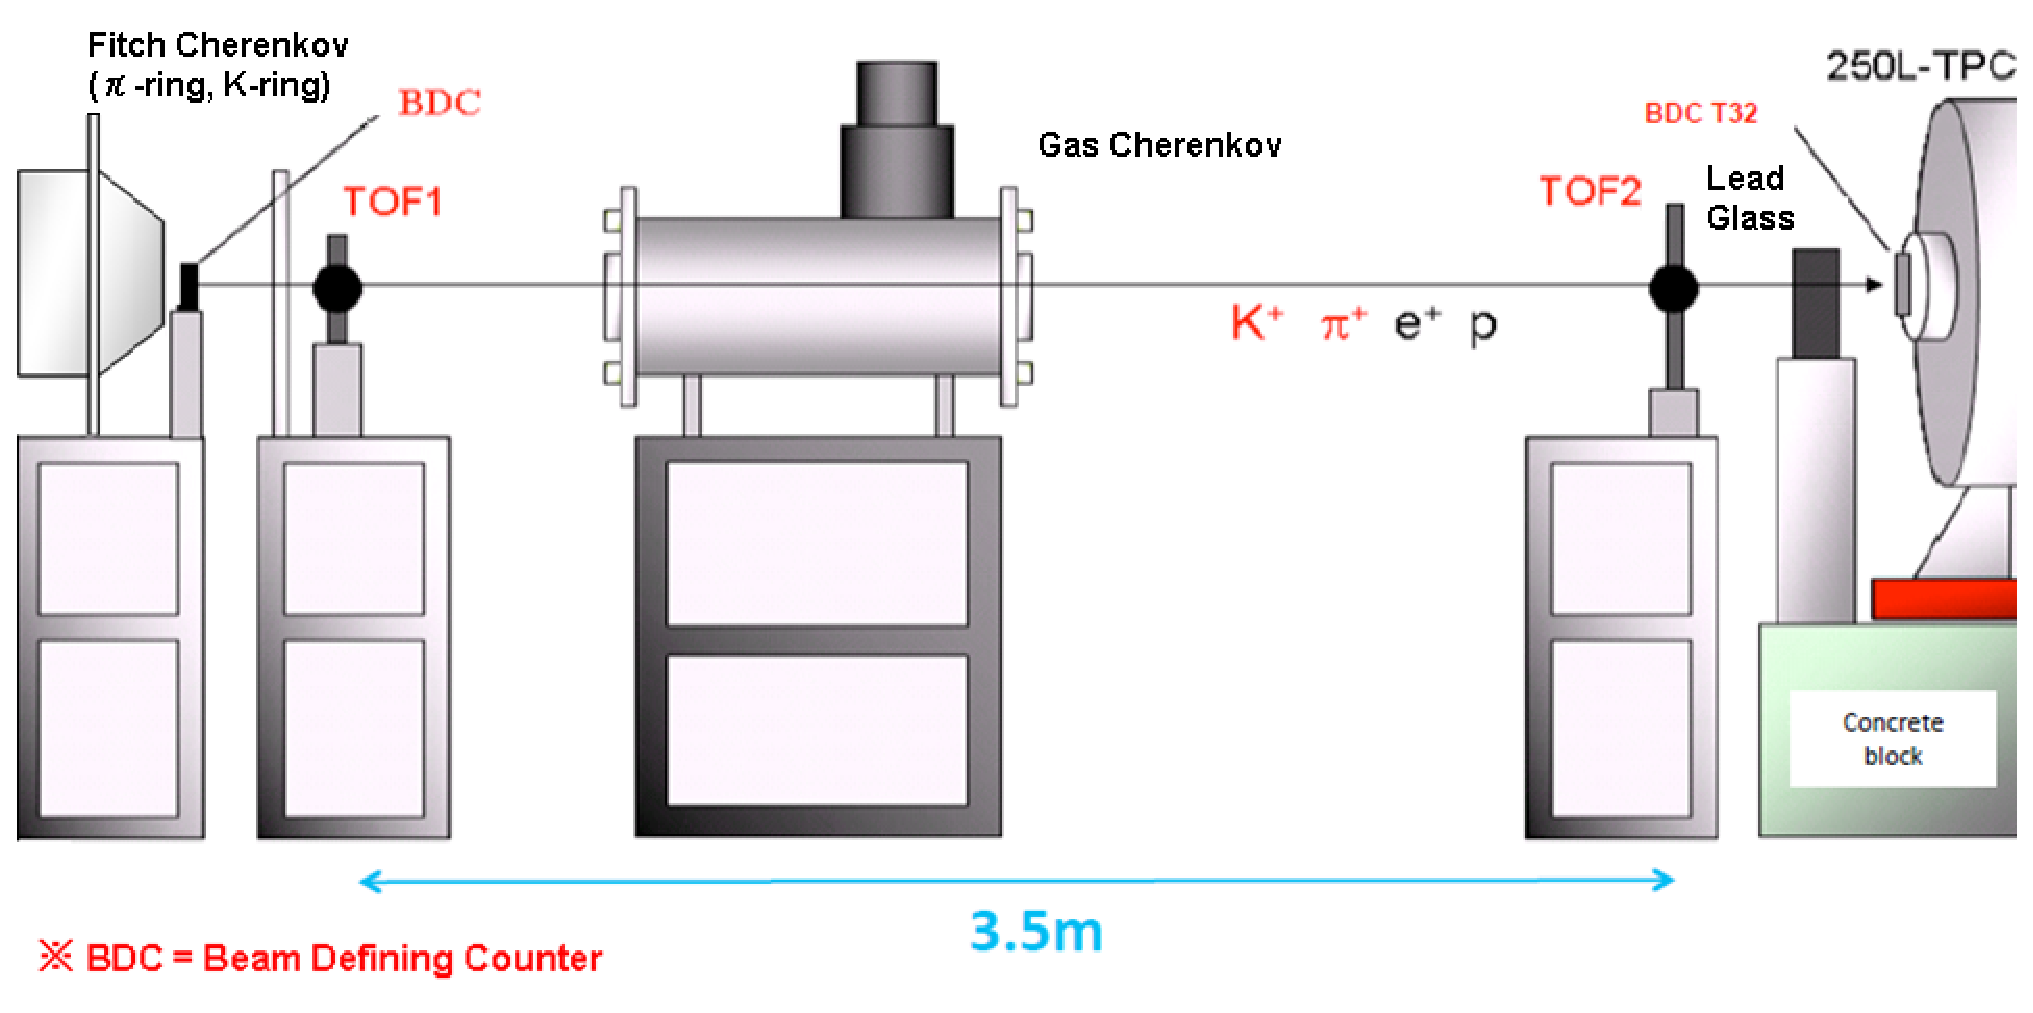
\includegraphics[width=1.0\hsize,clip]{fig/Beamline.eps}
%  \caption{Instruments on K1.1BR Beam Line}
%  \label{fig:Beamline}
%\end{figure}

Two TOF counters are 3.5m apart, and has $\sim$200 ps of time resolution.
Figure \ref{fig:BeamCountersTOF} shows the flight time distribution between TOF1 and TOF2
obtained from 800 MeV/$c$ beam particles which contain all $K^{+}$, $\pi{+}$, $e^{+}$, and $p$. 
Three peaks which correspond to $\pi$+$e^+$, $K^+$, and $p$, respectively, are well separated.

FC has 5 cm of acrylic plate as Cherenkov light radiator and 
photo-multipliers which are aligned in circles with two different emission angles
($K$-ring and $\pi$-ring) as photo detector.
It is designed to have maximum separation of $K^{+}$ and $\pi^{+}$ with momentum of 800 MeV/$c$.
Top plot in Fig.\ref{fig:BeamCountersFC} shows response of FC for the 800 MeV/$c$ beam particles. 
Horizontal axis and vertical axis are hit multiplicity of the $\pi$-ring and $K$-ring, respectively. 
$K^+$($\pi$) is identified as event with signal in $K$-ring ($\pi$-ring) but no signal in $\pi$-ring ($K$-ring).
In case of no signals in both rings, the particle is considered as proton.
TOF and FC can not distinguish $e^{+}$ and $\pi^+$
Additional separation between $e^{+}$ from $\pi^+$ is provided by GC which uses atmospheric air as
Cherenkov radiator. 
Filled histograms in bottom plot of Fig.\ref{fig:BeamCounters} shows selected $K^+$ event with FC information.
FC can identify $K^+$ with almost very high efficiency. After removing residual $\pi^+$ using TOF, we can obtain
almost 100\% purity $K^+$ sample.


\begin{figure}[htbp]
  \begin{center}
    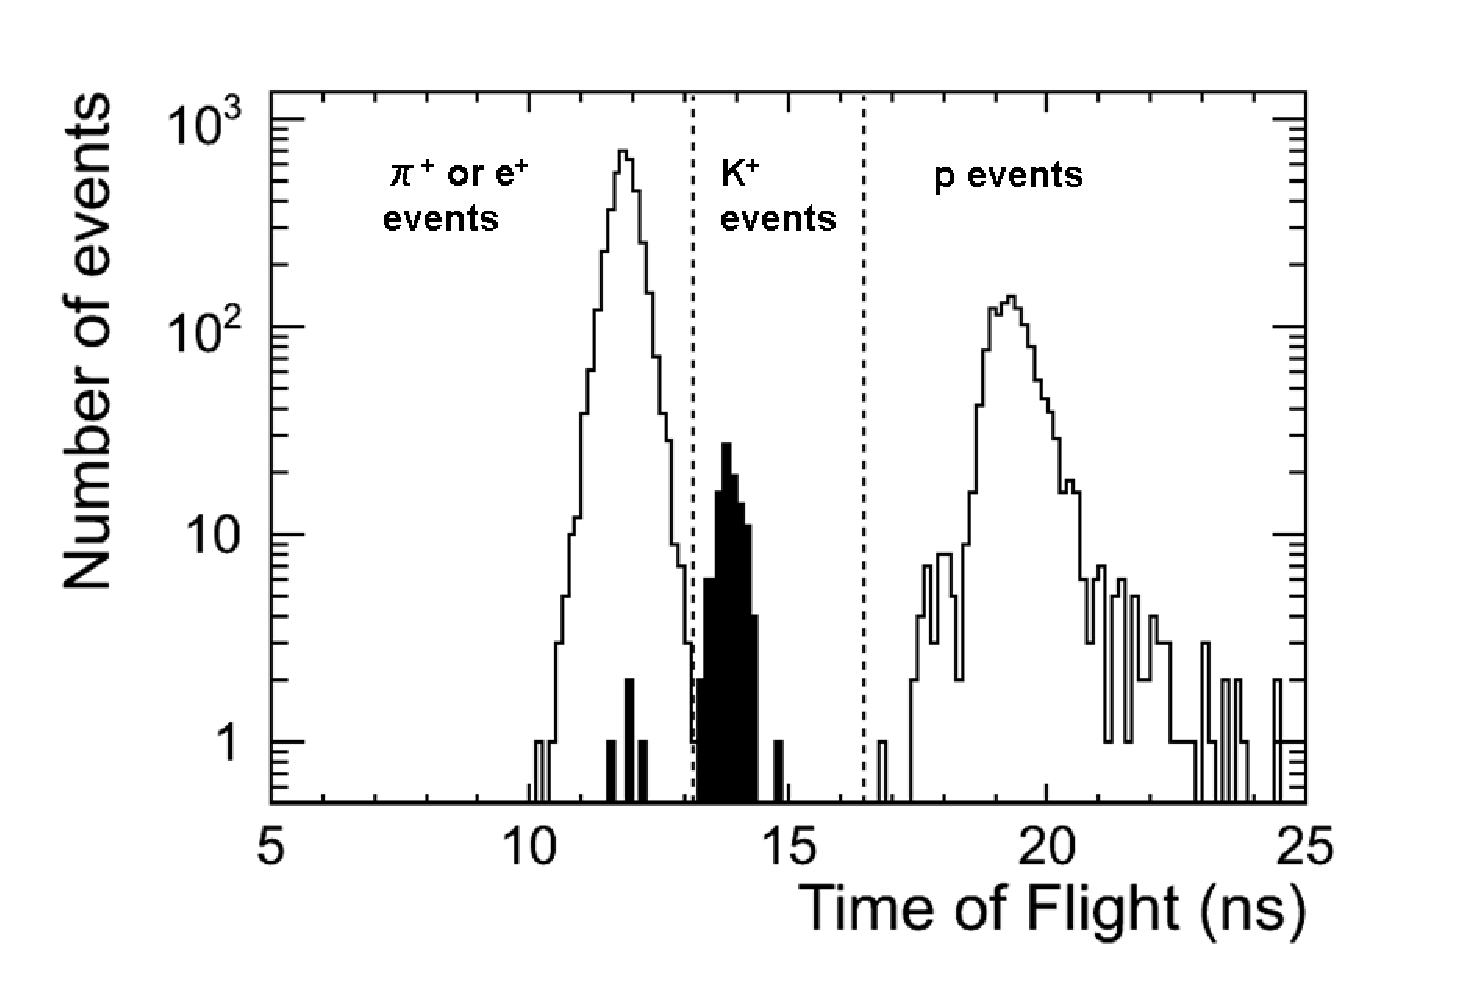
\includegraphics[width=1.0\hsize,clip]{fig/TOF_cut.eps}
  \end{center}
 \caption{TOF distribution.}
 \label{fig:BeamCountersTOF}
\end{figure}

\begin{figure}[htbp]
  \begin{center}
    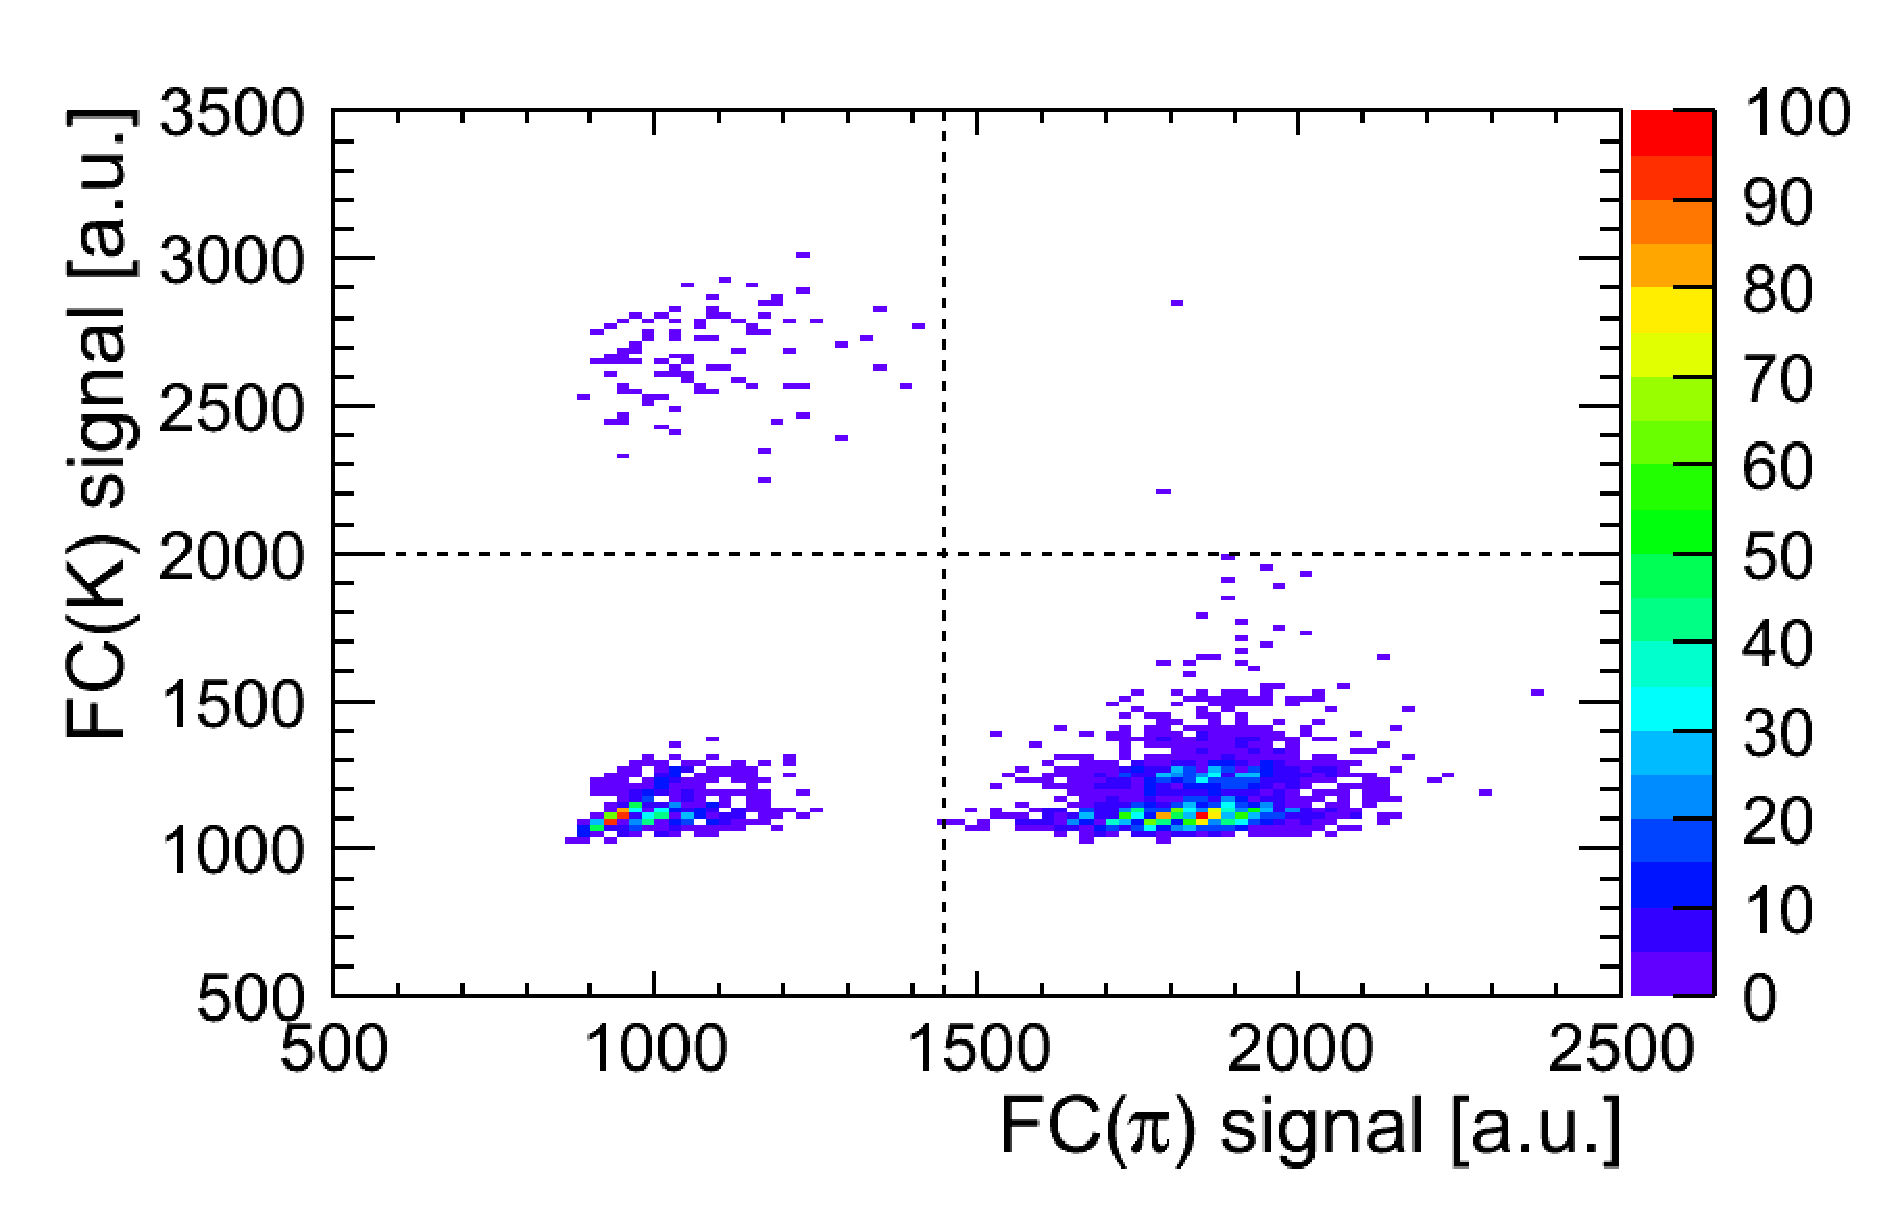
\includegraphics[width=1.0\hsize,clip]{fig/FC_KPI.eps}
  \end{center}
 \caption{FC}
 \label{fig:BeamCountersFC}
\end{figure}

\subsection{Oct/2010 Beam Test Configuration}

by using the beam counters, we define three types of trigger
\begin{itemize}
\item non-bias trigger:  simply require signal in two BDCs and two TOFs
\item Kaon trigger:  in addition to no-bias require K id with FC information  
\item electron trigger: non-bias + electron ID with GC information
\end{itemize}

Beam Momentum
\begin{itemize}
\item Materials located from proton target to LArTPC detector (beam counters, beam windows, air, etc) degrade beam particle momentum
\item the effect is estimated by looking at TOF of proton, average prton beam momentum is 730 MeV/$c$
\item For other particles  (K, pi,e e), TOF does not have enough resolution to determin momentum, and the degradation
is directly estimated by counting the energy deposition to the materials using GEANT based simulation.
For example Kaon momentum is xxx MeV/c on average.
\end{itemize}

\begin{figure}[htbp]
  \begin{center}
    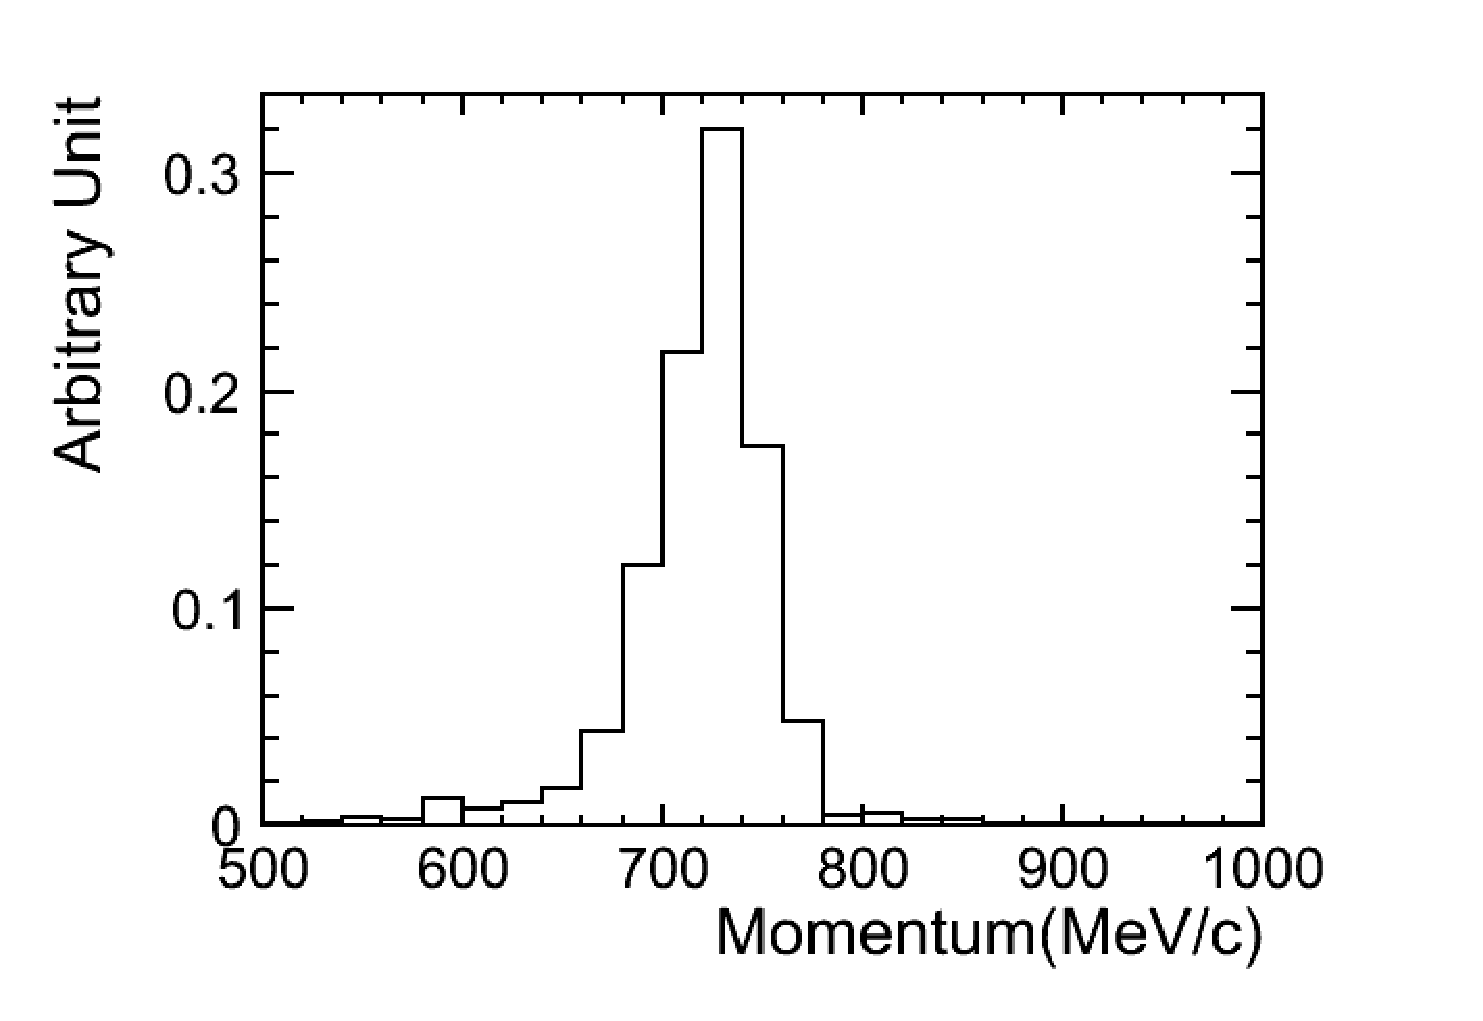
\includegraphics[width=1.0\hsize,clip]{fig/Momentum_proton.eps}
    \caption{Top plot shows $\rm {\Delta TOF}$ distribution of TOF counters with proton data,
      and bottom plot shows proton momentum estimated by $\rm {\Delta TOF}$ of TOF counters information}
    \label{fig:Proton_momentum}
  \end{center}
\end{figure} 

We measured beam profile in front of 250LAr TPC beam window by using plastic scintillation counters.
%Figure \ref{beamprofile_250L} shows the result.
The beam is relatively narrow in vertical direction (within 5 cm),
but spread in horizontal direction ($\sim$ 10 cm).

%\begin{figure}[!htb]
%  \begin{center}
%     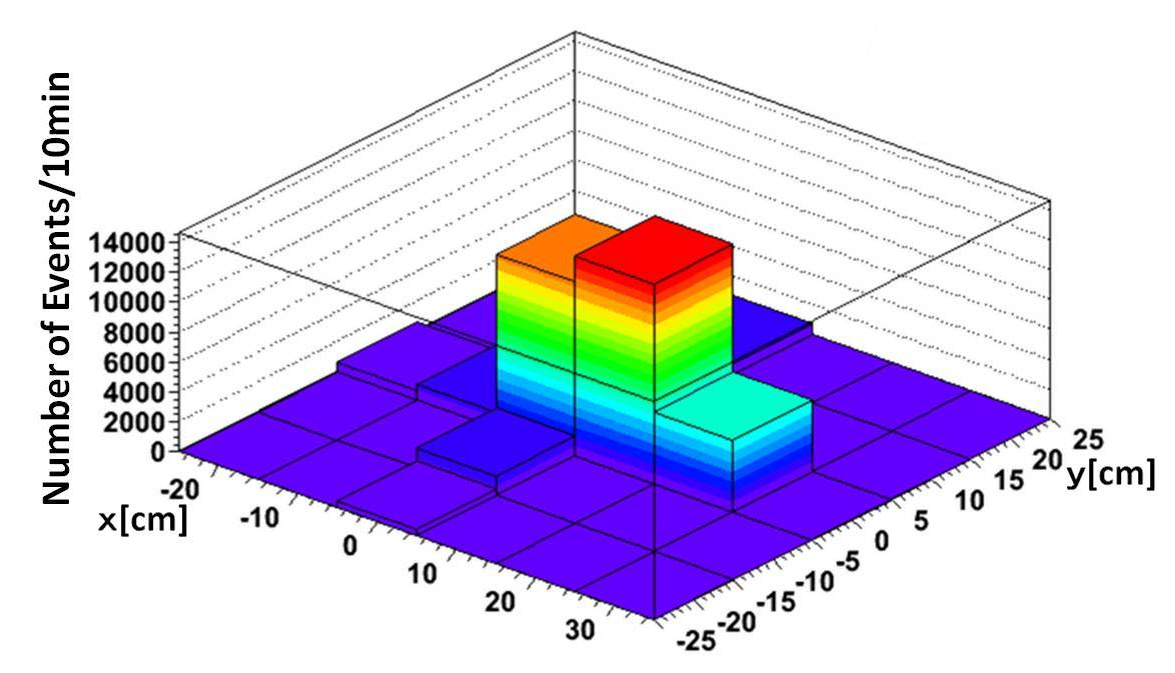
\includegraphics[width=0.8\hsize,clip]{./fig/BeamProfile3.eps}
%  \end{center}
%  \caption{Beam profile on the front of 250LAr TPC}
%  \label{beamprofile_250L}
%\end{figure}


